\documentclass{cup-pan}
\usepackage{blindtext}
\usepackage{comment}
\usepackage{setspace}
\spacing{1.15}
\renewcommand*\contentsname{Summary of the contents}
\subsectionfont{\color{PANDarkBlue}}

\title{Practical Coursework,\\ Video Game FanArt, \\ The Legend of Zelda: Breath of the Wild.}

\author{Jesus Jimenez Montero}

\affil[1] {Informática Básica, VJ1202}
\affil[2] {Expresión Artística, VJ1204}
\affil[3] {Inglés Moderno, VJ1205}

%% Corresponding author
\corrauthor{Jesús Jiménez Montero}

%% Abbreviated author list for the running footer
\runningauthor{Jesus JM}

\addbibresource{refs.bib}

\begin{document}

\maketitle
%\hrule
\textcolor{PANDarkBlue}{\hrule}


\tableofcontents
\newpage
\listoffigures
\newpage

\begin{abstract}
    This document is a practical coursework for the subject, "Informática Básica". It's a fanart of the video game, "The Legend of Zelda: Breath of the Wild". The main goal of this coursework is to adapt the Hero's Quest to the drawings.
    This document will be written in English due to the collaboration with the subject, "Inglés Moderno". 
    And the format of the document is done with the language LaTeX, and the template PAN (Template for submission to Political Analysis).

\end{abstract}

%%______________________________________________________________________________
%%______________________________________________________________________________

\section{Introduction}

    \textcolor{PANDarkBlue}{\large Description of the game}\\
    
    The Legend of Zelda, Breath of the Wild; is a video game exclusive to the Nintendo Switch console, released in 3rd March 2017. 
    Breath of the Wild is an open-world adventure game based on the world of Hyrule, 100 years after the battle that took place where Ganon was sealed in the castle of Hyrule with Zelda protecting the seal. Link is almost defeated on this battle and goes to a deep sleep.
    
    After 100 years as previously mentioned, he's woken up by a distant Zelda from its dormancy and goes out of the cave he was staying at, greeted by a distant and sisnister Hyrule Castle. And the adventure can begin!\\
    
    \textcolor{PANDarkBlue}{\large Adaptation of the hero's quest}\\
    One of the requirements for this coursework was to adapt the Hero's Quest to the drawings.
    To make my drawings accomplish this task, I used the key points of Link's Adventure, being:\\
        \begin{enumerate}
            \item After the extended tutorial where Link's gets its paraglider to get down the plateau where the game begins and one of the first things the player does is look to the Dueling Peaks, one of the key points on the game, where Link discovers its true quest.\\
            \item Where the player gains its confidence to destroy a Guardian, whose quest is to keep out intruders from key areas. This also a key point of the game because destroying a guardian means you are one step closer to defeating Ganon. \\
            \item ESTE PUNTO HACE FALTA COMPLETARLO YA QUE NO TENGO NINGUN DIBUJO, tiene que ser del ultimo fan art, en concreto de un key point de la historia que sea ultimo del juego. \\
        \end{enumerate}

%%______________________________________________________________________________
%%______________________________________________________________________________

\section{Reference images}

    For the references used in the project, I used a combination of images from the game (to make it as accurate as possible), some images from internet and the most important part, 3D renders made in Bldner with the stuff that appears on the fanarts. 

    \subsection*{Images from the game}
    Beginning with the captures of the game, for the Dueling Peaks, I used the following image:\\
    \begin{figure}[H]
        \includegraphics[width=0.5\textwidth]{Imagenes/Referencias/article_img03_1.jpg}
        \caption{Image reference of the Dualing Peaks}
    \end{figure}
    This image gave me the point of reference to create the player on the hill. 

    And this image: 
    \begin{figure}[H]
        \includegraphics[width=0.5\textwidth]{Imagenes/Referencias/Dueling_Peaks.png}
        \caption{The Dueling Peaks with the bridge near the enemy camp}
    \end{figure}
    This image was also very important in the creation of the fanart, because it was the biggest reference point of the Dueling Peaks.\\

    \subsection*{3D Renders}
    I also used 3D renders to make the fanarts, because my area of expertise is 3D, and I wanted to take advantage of this.
    So first, a simple blocks rig
    (\footnote{Rig made by 
    \href{https://hozq3d.gumroad.com/l/Blocks}{hozq3d}}) 
    was used to pose the character: 
    \begin{figure}[H]
        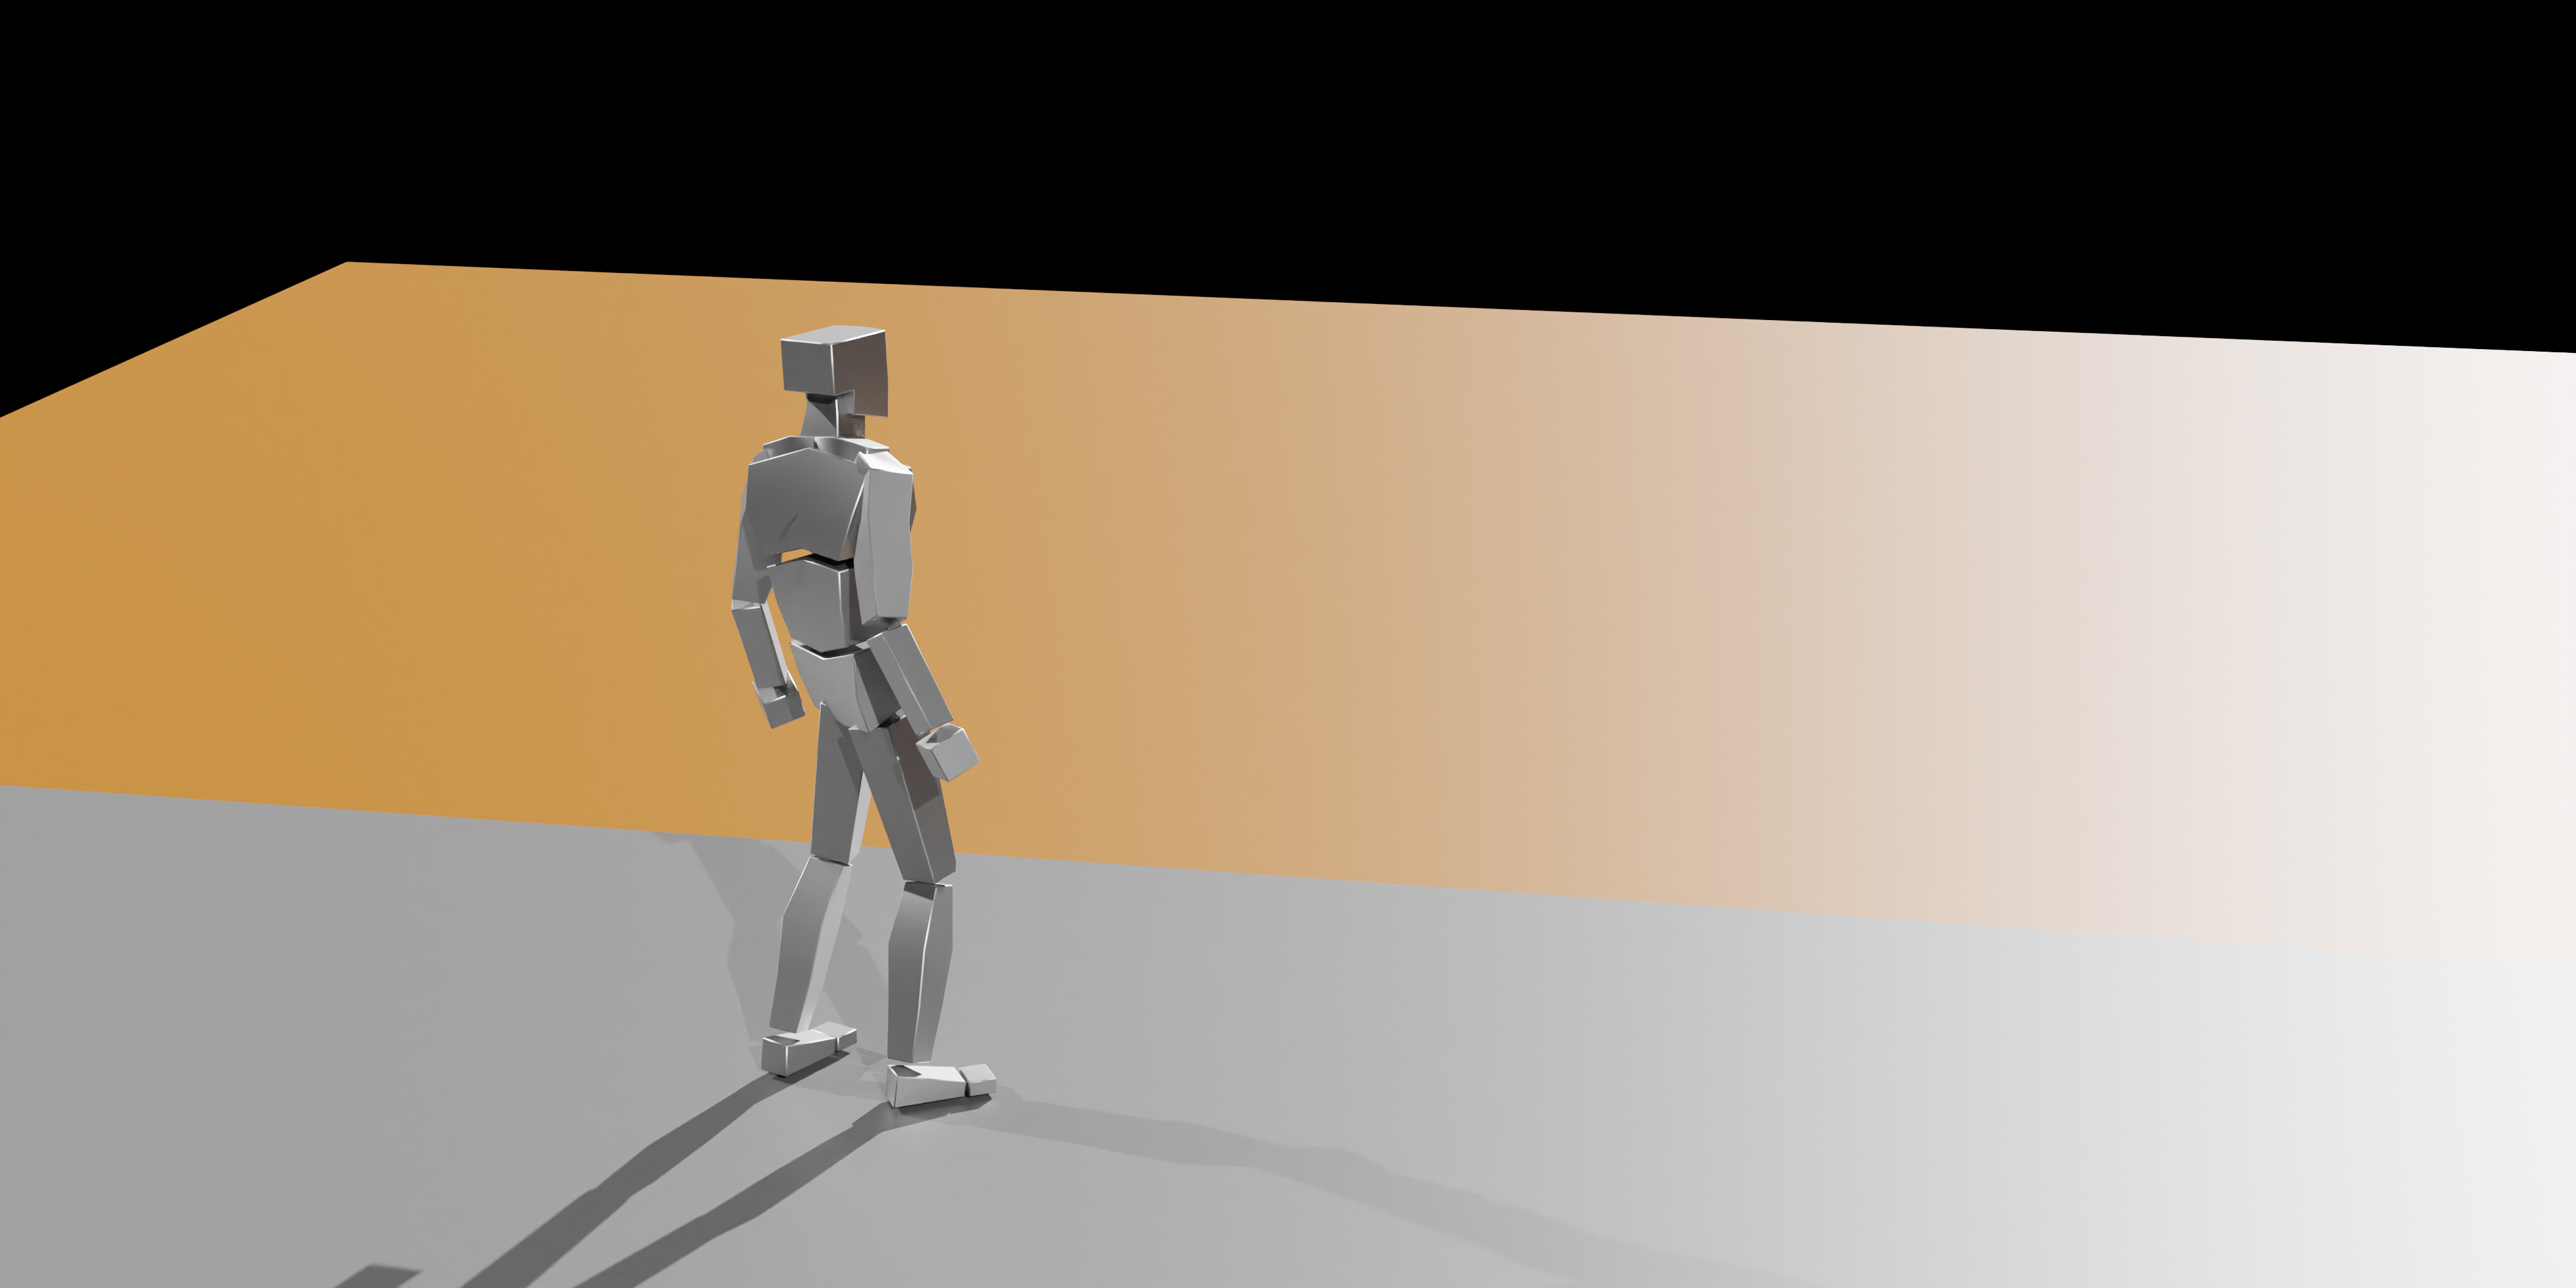
\includegraphics[width=0.5\textwidth]{Imagenes/Referencias/renefernce_3d_3.png}
        \caption{Blocks rig}
    \end{figure}

    And then, a rig of Zelda was used to pose the final character and have more detail:    
    (\footnote{Rig made by 
    \href{https://www.youtube.com/watch?v=1EUcGBMVRbA}{Soranin} and ported to Blender by  
    \href{https://twitter.com/mehaloArt/status/1528197222751383552?s=20}{mehaloArt}})

    \begin{figure}[H]
        \includegraphics[width=0.5\textwidth]{Imagenes/Referencias/ref_zelda.png}
        \caption{Zelda rig}
    \end{figure}

    The Zelda Rig was also used in combination with another rig, which was a Guardian 
    (\footnote{Rig made by 
        \href{https://sketchfab.com/3d-models/guardian-zelda-botw-fan-art-990a6a9434c849329360ea1ef9078895}{NinKorr3D}}), to make the final fanart.
    \begin{figure}[H]
        \includegraphics[width=0.5\textwidth]{Imagenes/Referencias/referencia art 2.png}
        \caption{Zelda and the Guardian Rig}
    \end{figure}

    The usage of manually created 3D renders allowed for a much diverse expression of the fan arts, allowing a preview of how the final fan art would look like and facilitating the creation process.\\

%%______________________________________________________________________________
%%______________________________________________________________________________

\section{Analysis of formal elements of a concept art}
    \begin{figure}[H]
       \includegraphics[width=0.5\textwidth]{Imagenes/Referencias/conceptart_a_analizar.png}
        \caption{Concept art to analyze}
    \end{figure}

%%______________________________________________________________________________
%%______________________________________________________________________________
\begin{comment}
    Distintos dibujos de evolución, dibujos descartados y resultado final
    acompañados de texto explicativo sobre la acción que representa la ilustración y también los
    elementos formales utilizados
\end{comment}

\newpage
\section{First Illustration}
    \subsection{Line art and sketches}

    \subsection{Chiaroscuro}

    \subsection{Coloring}

    \subsection{Final Result}
\newpage
%%______________________________________________________________________________
%%______________________________________________________________________________
\newpage
\section{Second Illustration}

    \subsection{Line art and sketches}

    \subsection{Chiaroscuro}

    \subsection{Coloring}

    \subsection{Final Result}
\newpage
%%______________________________________________________________________________
%%______________________________________________________________________________
\newpage
\section{Third Illustration}

    \subsection{Line art and sketches}

    \subsection{Chiaroscuro}

    \subsection{Coloring}

    \subsection{Final Result}
    \newpage
%%______________________________________________________________________________
%%______________________________________________________________________________
\newpage
\section{Conclusions}

    \subsection{Line art and sketches}

    \subsection{Chiaroscuro}

    \subsection{Coloring}

    \subsection{Final Result}
\newpage

\end{document}